\documentclass[a4paper,11pt]{article}
\usepackage[paper=a4paper, left=1.5cm, right=1.5cm, bottom=1.5cm, top=1.5cm]{geometry}
\usepackage{ucs}
\usepackage[utf8x]{inputenc}
\usepackage{amsmath}
\usepackage{amsfonts}
\usepackage{amssymb}
\usepackage{amsthm}
\usepackage[latin,spanish]{babel}
\usepackage{fontenc}
\usepackage{graphicx}
\usepackage{cancel}
% \usepackage{algpseudocode}
% \usepackage{algorithmicx}
% \usepackage{color}
% \usepackage{pdfpages}
% \usepackage{tikz}
%%%%%% Si se usa tikz para dibujar digrafos, cuando pongas flechas, tira un conflicto. Se soluciona con estas dos lineas:
% \usepackage[matrix,arrow]{xy}
% \usetikzlibrary{intersections}

\usepackage{dsfont}
\newcommand{\real}{\mathds{R}}
% \newcommand{\nat}{\mathds{N}}
% \newcommand{\complejos}{\mathds{C}}
% \newcommand{\Subesp}{\mathds{S}}

\usepackage{hyperref}
\hypersetup{%
 % Para que el PDF se abra a pagina completa.
  pdfstartview= {FitH \hypercalcbp{\paperheight-\topmargin-1in-\headheight}},
  pdfauthor={Gaston Requeni},
  pdfsubject={Preinforme - Final Orga2},
 %pdfkeywords={keyword1} {key2} {key3},
 colorlinks=true,
  linkcolor=black,
  urlcolor=blue
}

\author{Gastón Requeni}
\title{Reconocimiento de Patrones\\ Trabajo Práctico 1\\ Clasificador Bayesiano}
\date{DD/MM/AAAA}


\parskip = 4pt


\begin{document}
\maketitle

\section{Introducción}
Sea el conjunto de datos $\mathcal{D} = \{(x_1,t_1), \dots, (x_N,t_N)\}$, siendo $x_i\in\real^D$ un feature vector y $t_i\in \{\mathcal{C}_1, \dots, \mathcal{C}_K\}$ la clase del vector $x_i$. Además asumimos conocidas las distribuciones de los datos de cada clase (verosimilitudes) y probabilidades a priori, es decir que:
\begin{itemize}
  \item $p_X(x|T = C_k)$ es conocida para todo $k=1\dots K$, siendo $X$ la variable aleatoria contínua que genera los feature vectors, $T$ la variable aleatoria cuyo rango es $R_T = \{\mathcal{C}_1, \dots, \mathcal{C}_K\}$ y $p_X(x|T = C_k)$ es la función de densidad de probabilidad (pdf) contínua de $X$ condicional a $T$ (verosimilitud). Notación: $p(x|C_k)$.
  \item $P(T=C_k)$ es conocida para todo $k=1\dots K$, siendo $P(T=C_k)$ la probabilidad puntual de $T$ (probabilidad a priori). Notación: $P(C_k)$.
\end{itemize}

El clasificador Bayesiano calcula las probabilidades a posteriori ($P(T=C_k|X=x) = P(C_k|x)$) utilizando el teorema de Bayes:
$$P(C_k|x) = \frac{p(x|C_k) P(C_k)}{p(x)}$$
donde $p(x)=\sum_{k=1}^{K} p(x|C_k)P(C_k)$ (evidencia).
Luego dado un nuevo $x\in\real^D$, se clasifica en la clase de mayor probabilidad a posteriori, es decir se asigna la clase $C_k$ tal que:
$$ P(C_k|x) \geq P(C_i|x) \ \ \forall i=1\dots K$$
Dado que el término $p(x)$ aparece dividiendo de ambos lados de la desigualdad (y es positivo), se puede cancelar, quedando como discriminante:
$$g_i(x) = p(x|C_k) P(C_k)$$
Luego se elige la clase $k = \arg \max_{i=1}^{K} g_i(x)$.

Cuando las verosimilitudes y probabilidades a priori son desconocidas, se pueden usar estimadores de máxima verosimilitud, asumiendo que $p(x|C_k)\sim\mathcal{N}(\mu_k, \Sigma_k)$: Sean $\{y_1,\dots, y_{N_k}\} \subset \{x_1,\dots, x_N\}$ los datos correspondientes a la clase $C_k$,
\begin{itemize}
  \item $P(C_k) \approx \frac{N_k}{N}$
  \item $\mu_k \approx \frac{1}{N_k} \sum_{i=1}^{N_k} y_i$
  \item $\Sigma_k \approx \frac{1}{N_k} \sum_{i=1}^{N_k} (y_i - \mu_k)(y_i - \mu_k)^t = \frac{1}{N_k} MM^t$, con
  $col_i(M) = (y_i - \mu_k) \ \forall i=1\dots N_k$. 
\end{itemize}

\newpage

\section{Ejercicio 1: Ejemplos de clasificadores Bayesianos para $D=2, K=2$.}

Vamos a analizar casos donde $p(x|C_1)\sim\mathcal{N}(\mu_1, \Sigma_1)$ y $p(x|C_2)\sim\mathcal{N}(\mu_2, \Sigma_2)$, siendo $\mu_1,\mu_2\in\real^2$ y $\Sigma_1,\Sigma_2\in\real^{2\times 2}$. Además vamos a asumir que $P(C_1)=P(C_2)=0.5$.

\subsection*{Caso 1: $\Sigma_1 = \Sigma_2 \propto I$}
Tomamos $\mu_1 = (0;0)^t, \ \ \mu_2 = (2.5; 4.5)^t$ y $\Sigma_1=\Sigma_2 = \begin{pmatrix}2 & 0\\ 0 & 2 \end{pmatrix}$.

\begin{figure}[h!]
\centering
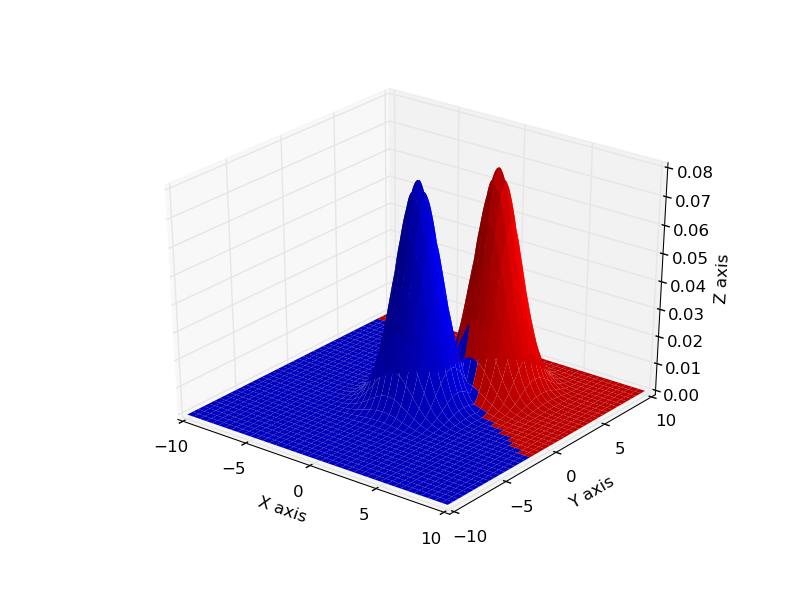
\includegraphics[width=0.45\textwidth]{img/ej1-caso1-pdf.png}
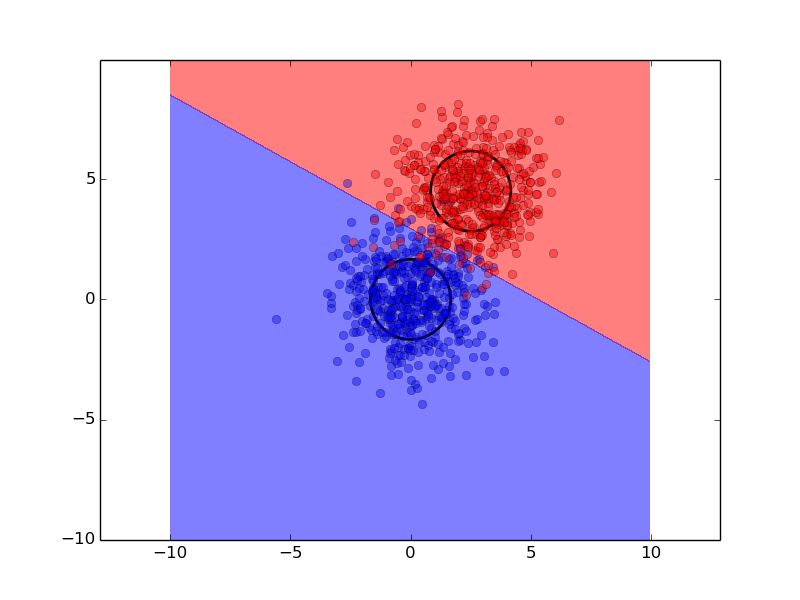
\includegraphics[width=0.45\textwidth]{img/ej1-caso1-region.png}
\caption{A la izquierda las pdfs y a la derecha las regiones de clasificación resultantes, con algunos puntos de ejemplo. En azul $C_1$ y en rojo $C_2$.}
\label{ej1_caso1}
\end{figure}

Como puede observarse en la Figura \ref{ej1_caso1}, al tener una matriz de covarianzas proporcional a la identidad, se obtienen los puntos en forma de circunferencia y la frontera es una recta.


\subsection*{Caso 2: $\Sigma_1 = \Sigma_2 \  \cancel{\propto} \  I$}
Tomamos $\mu_1 = (0;0)^t, \ \ \mu_2 = (2.5; 4.5)^t$ y $\Sigma_1=\Sigma_2 = \begin{pmatrix}\sigma_1^2 & \rho\sigma_1\sigma_2 \\ \rho\sigma_1\sigma_2 & \sigma_2^2 \end{pmatrix}$, siendo $\sigma_1 = \sqrt{2}, \sigma_2 = 2, \rho=-0.6 $.

\begin{figure}[h!]
\centering
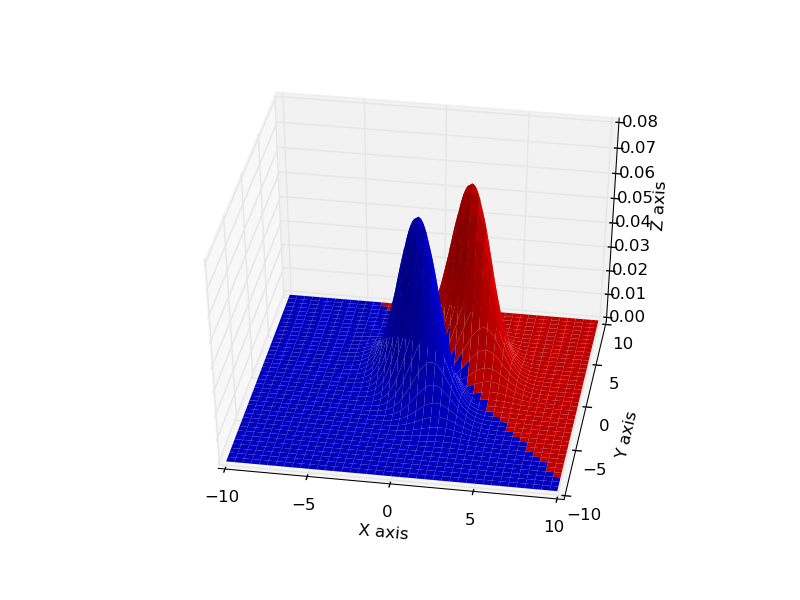
\includegraphics[width=0.45\textwidth]{img/ej1-caso2-pdf.png}
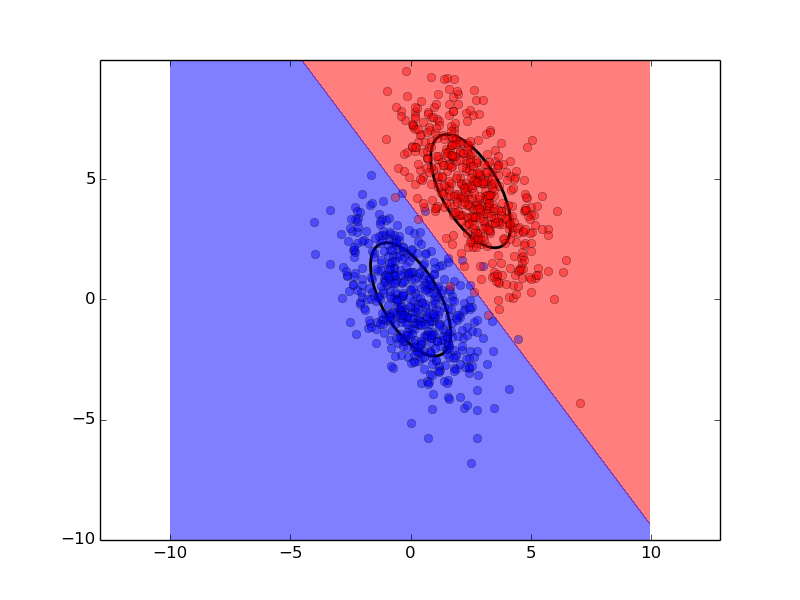
\includegraphics[width=0.45\textwidth]{img/ej1-caso2-region.png}
\caption{A la izquierda las pdfs y a la derecha las regiones de clasificación resultantes, con algunos puntos de ejemplo. En azul $C_1$ y en rojo $C_2$.}
\label{ej1_caso2}
\end{figure}

Como puede observarse en la Figura \ref{ej1_caso2}, al tener una matriz de covarianzas que no es proporcional a la identidad, aparecen términos cruzados en las ecuaciones y los datos aparecen como en un elipse. Dado que ambas clases tienen la misma matriz de covarianzas, nuevamente la frontera es una recta.


\subsection*{Caso 3: $\Sigma_1 \neq \Sigma_2$}
En todos los casos, tomamos $\Sigma_k=\begin{pmatrix}(\sigma_1^{(k)})^2 & \rho^k\sigma_1^{(k)}\sigma_2^{(k)} \\ \rho^{(k)}\sigma_1^{(k)}\sigma_2^{(k)} & (\sigma_2^{(k)})^2 \end{pmatrix}$.
\subsubsection*{Hipérbola}
Tomamos $\mu_1 = (-2;-4)^t, \ \ \mu_2 = (2.5; 4.5)^t$, y $\Sigma_k$ definida por:
\begin{itemize}
  \item $\sigma_1^{(1)} = 3, \sigma_2^{(1)} = 2, \rho^{(1)}=0.6 $.
  \item $\sigma_1^{(2)} = \sqrt{2}, \sigma_2^{(2)} = 2, \rho^{(2)}=-0.6 $.
\end{itemize}

\begin{figure}[h!]
\centering
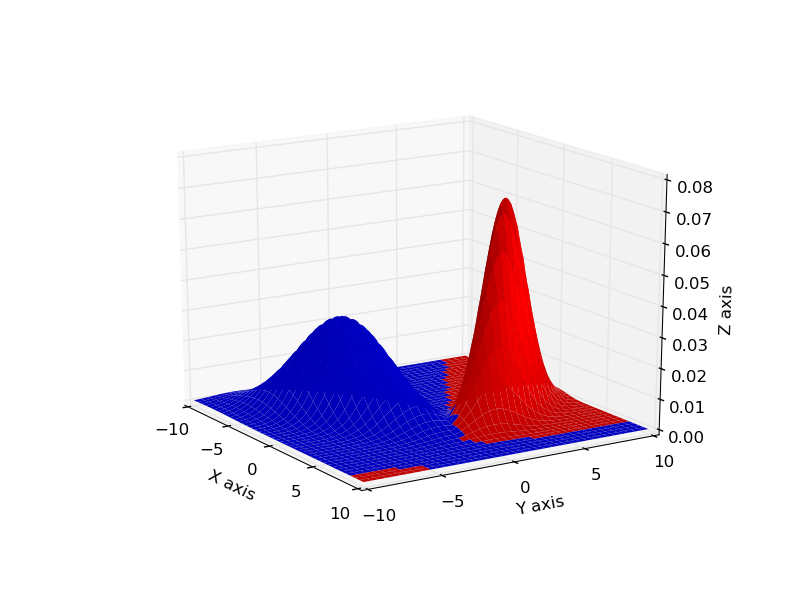
\includegraphics[width=0.45\textwidth]{img/ej1-caso3a-pdf.png}
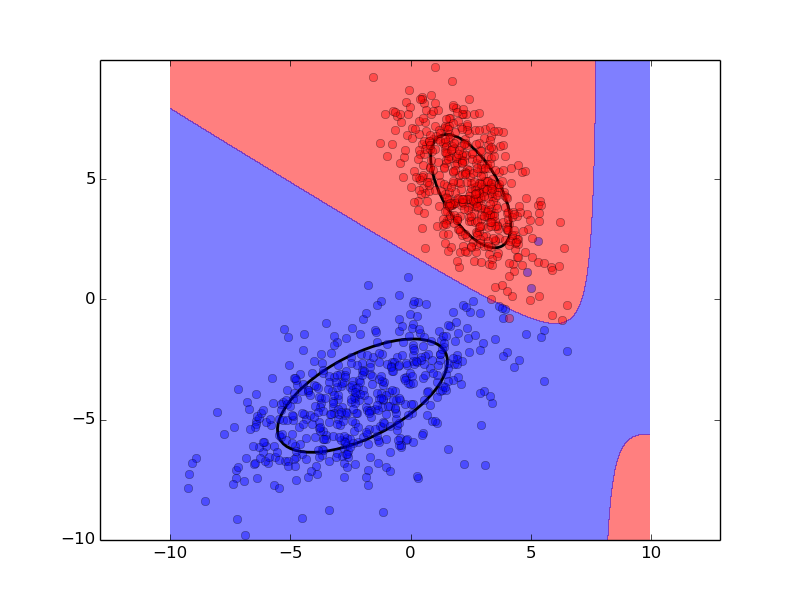
\includegraphics[width=0.45\textwidth]{img/ej1-caso3a-region.png}
\caption{A la izquierda las pdfs y a la derecha las regiones de clasificación resultantes, con algunos puntos de ejemplo. En azul $C_1$ y en rojo $C_2$.}
\label{ej1_caso3a}
\end{figure}

En la Figura \ref{ej1_caso3a} $C_2$ es la misma del {\bf Caso 2} y a $C_1$ le cambiamos el sentido de la correlación y agregamos dispersión en $\sigma_1$. Esto provoca que la frontera resultante sea una hipérbola.

\subsubsection*{Elipse}
Tomamos $\mu_1 = (0.5;-5)^t, \ \ \mu_2 = (0; 4.5)^t$ y $\Sigma_k$ definida por:
\begin{itemize}
  \item $\sigma_1^{(1)} = 3, \sigma_2^{(1)} = 2, \rho^{(1)}=0.2 $.
  \item $\sigma_1^{(2)} = 1, \sigma_2^{(2)} = 0.5, \rho^{(2)}=-0.3 $.
\end{itemize}

\begin{figure}[h!]
\centering
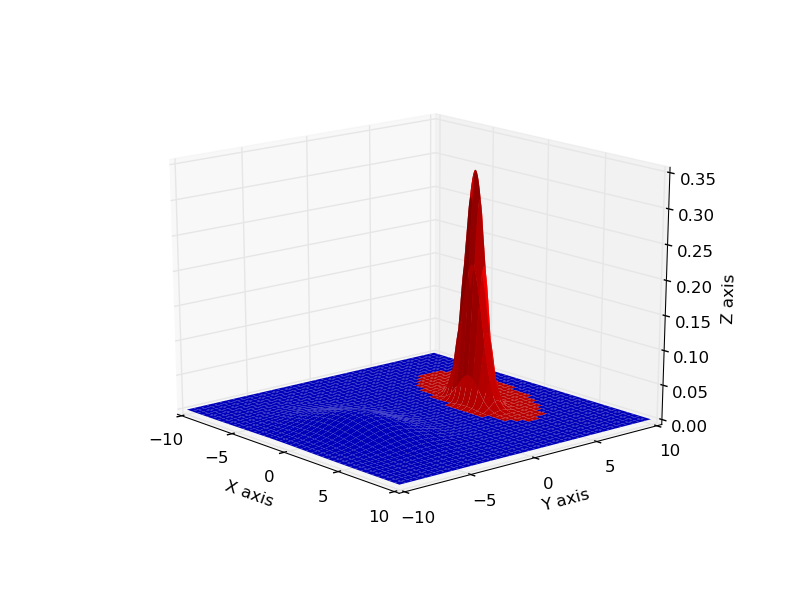
\includegraphics[width=0.45\textwidth]{img/ej1-caso3b-pdf.png}
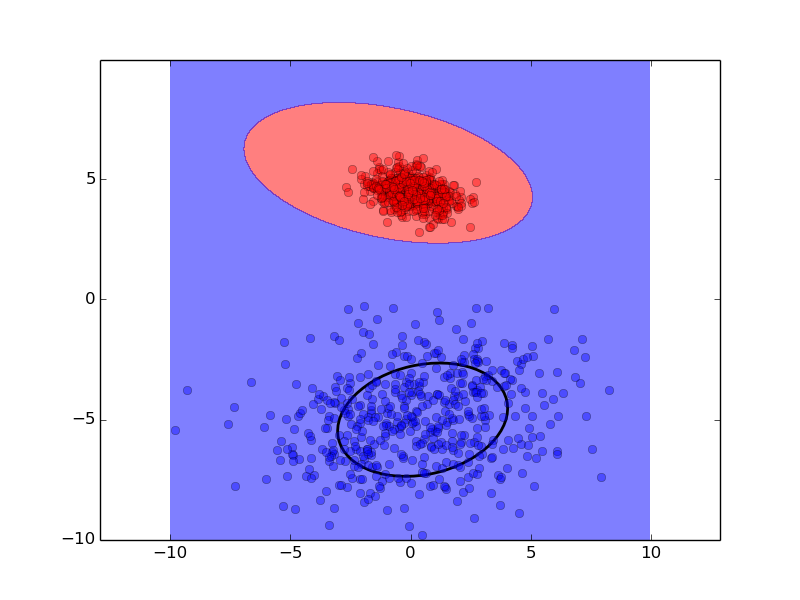
\includegraphics[width=0.45\textwidth]{img/ej1-caso3b-region.png}
\caption{A la izquierda las pdfs y a la derecha las regiones de clasificación resultantes, con algunos puntos de ejemplo. En azul $C_1$ y en rojo $C_2$.}
\label{ej1_caso3b}
\end{figure}

\newpage
En la Figura \ref{ej1_caso3b} se observa que la frontera es una elipse dado que $C_1$ (azul) tiene mucha dispersión en comparación con $C_2$ (rojo) que tiene muy poca.


\subsubsection*{Círculo ($\mu_1 = \mu_2$, $\Sigma_k \propto I$, $\Sigma_1 \neq \Sigma_2$)}
Tomamos $\mu_1 = \mu_2 = (0;0)^t$ y $\Sigma_k$ definida por:
\begin{itemize}
  \item $\sigma_1^{(1)} = 2, \sigma_2^{(1)} = 2, \rho^{(1)}=0 $.
  \item $\sigma_1^{(2)} = 5, \sigma_2^{(2)} = 5, \rho^{(2)}=0 $.
\end{itemize}

\begin{figure}[h!]
\centering
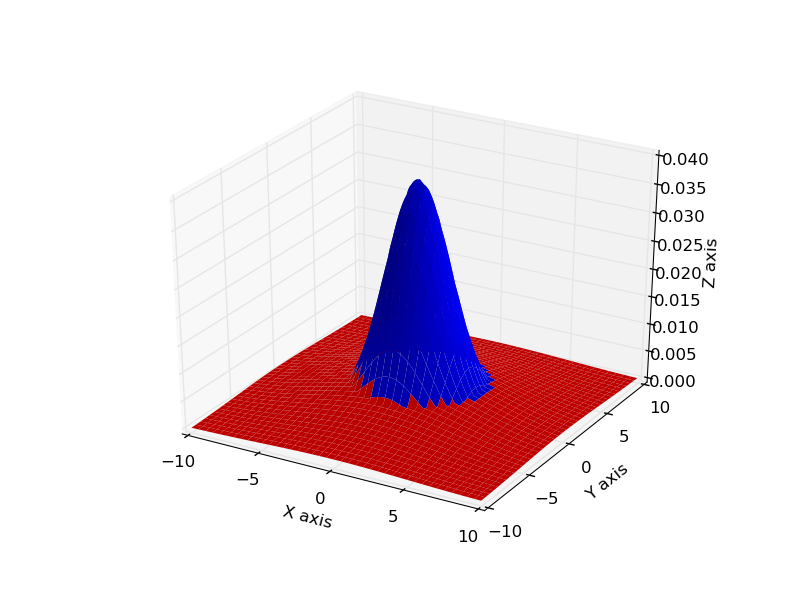
\includegraphics[width=0.45\textwidth]{img/ej1-caso3c-pdf.png}
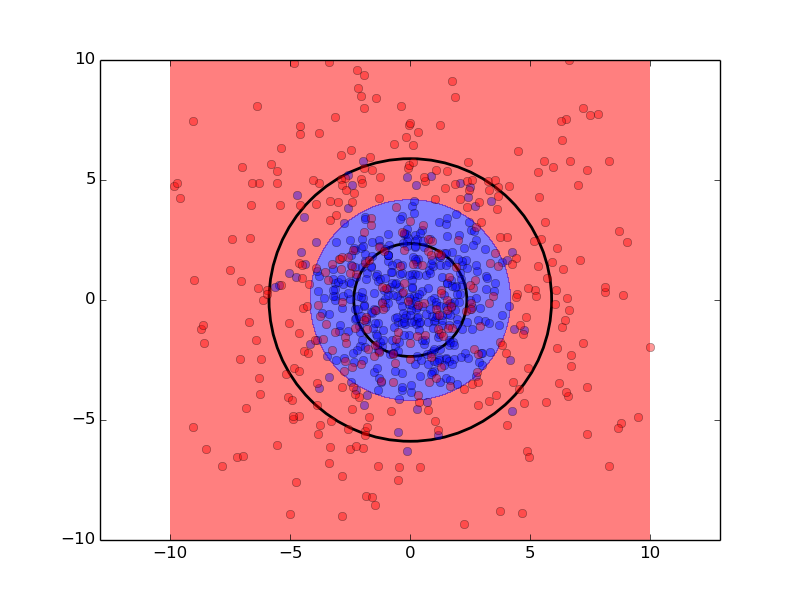
\includegraphics[width=0.45\textwidth]{img/ej1-caso3c-region.png}
\caption{A la izquierda las pdfs y a la derecha las regiones de clasificación resultantes, con algunos puntos de ejemplo. En azul $C_1$ y en rojo $C_2$.}
\label{ej1_caso3c}
\end{figure}

En la Figura \ref{ej1_caso3c} se observa que la frontera es un círculo. Observar que al tener $\mu_1 = \mu_2$ hay muchos puntos de $C_2$ (rojo) que están mal clasificados (dentro del círculo azul) y unos pocos de $C_1$ mal clasificados (los que caen fuera del círculo azul). El hecho de que la frontera sea un círculo se debe a que las covarianzas son proporcionales a la identidad entonces las distribuciones son simétricas y concentran los puntos en una circunferencia alrededor de la media.




\section{Ejercicio 2: Clasificación de imagenes sintéticas}

\begin{figure}
\centering
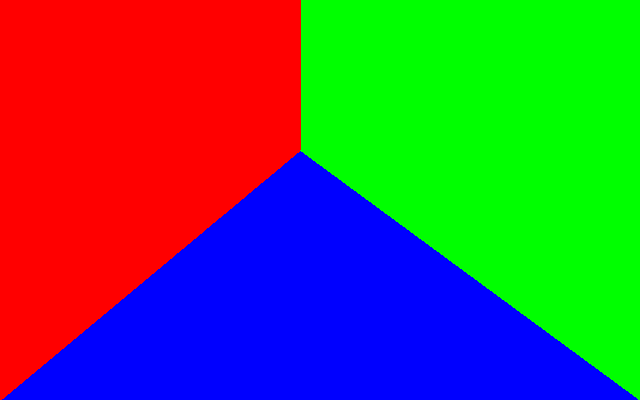
\includegraphics[width=0.45\textwidth]{img/phantomCustom.png}
\caption{Phantom de 3 clases utilizado. $C_1$ clase roja, $C_2$ clase verde, $C_3$ clase azul.}
\label{phantom}
\end{figure}

En este ejercicio vamos a utilizar una imagen \emph{phantom} de 3 clases (ver Figura \ref{phantom}). Eligiendo $\mu_i$ y $\Sigma_i$ para cada clase,
generaremos una \emph{imagen sintética} de la siguiente manera:
$$ ImSint(i,j) = random\_sample(\mathcal{N}(\mu_k, \Sigma_k)), \ \ \ \text{con } C_k = Phantom(i,j)$$
Es decir que en cada pixel $(i,j)$ vamos a guardar una muestra aleatoria correspondiente a la clase que indica el phantom para ese pixel.

Luego vamos a construir un clasificador Bayesiano utilizando los $(\mu_i, \Sigma_i)$ conocidos y vamos a clasificar los pixels de la imagen sintética.
Con esta clasificación vamos a armar una \emph{imagen clasificada}, donde cada pixel tendrá el color de la clase $C_k$ que le asignó el clasificador Bayesiano. El color de cada clase es el mismo color que usaba el phantom. De esta manera podemos visualizar el ruido generado al clasificar en función de $(\mu_i, \Sigma_i)$. Además calcularemos la matriz de confusión (o tabla de contingencia) para estudiar la eficiencia del método en cada caso.

En todos los casos asumimos que las clases son equiprobables a priori ($P(C_1) = P(C_2) = P(C_3)$).

\subsection*{Caso 1: $\Sigma_1 = \Sigma_2 = \Sigma_3 \propto I$}
Veamos dos ejemplos. En el primero, tomamos las medias muy cercanas y en el segundo las separamos un poco. En ambos casos tomamos:
$\Sigma_k = \begin{pmatrix}3 & 0\\ 0 & 3\end{pmatrix}$. Recordar que $C_1$ es la clase roja, $C_2$ es la clase verde y $C_3$ es la clase azul.
\begin{enumerate}
  \item $\mu_1 = (1;1)^t$, $\mu_2 = (1.5; 1.5)^t$, $\mu_3 = (2;2)^t$ (ver Figura \ref{ej2_caso1a})
  \item $\mu_1 = (0;0)^t$, $\mu_2 = (3; 3)^t$, $\mu_3 = (6;6)^t$ (ver Figura \ref{ej2_caso1b})
\end{enumerate}

\begin{figure}[h!]
\centering
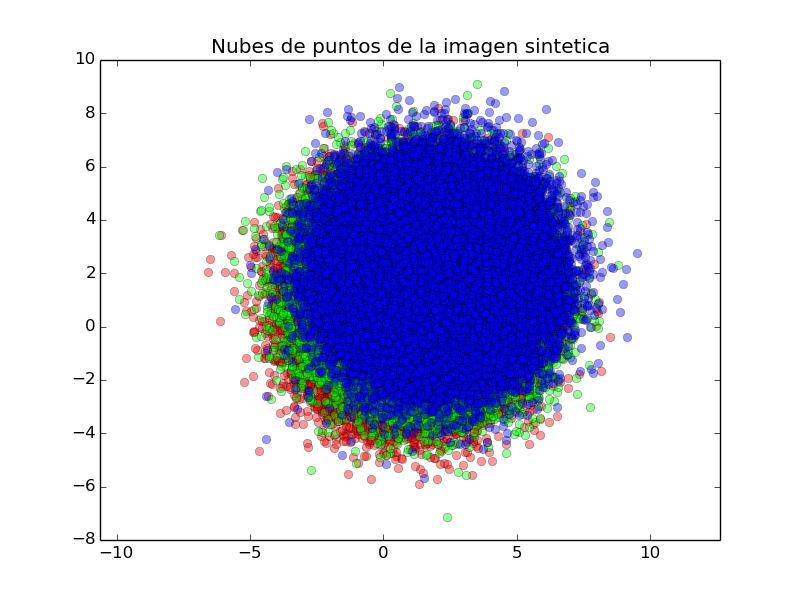
\includegraphics[width=0.45\textwidth]{img/ej2-caso1a-puntos.png}
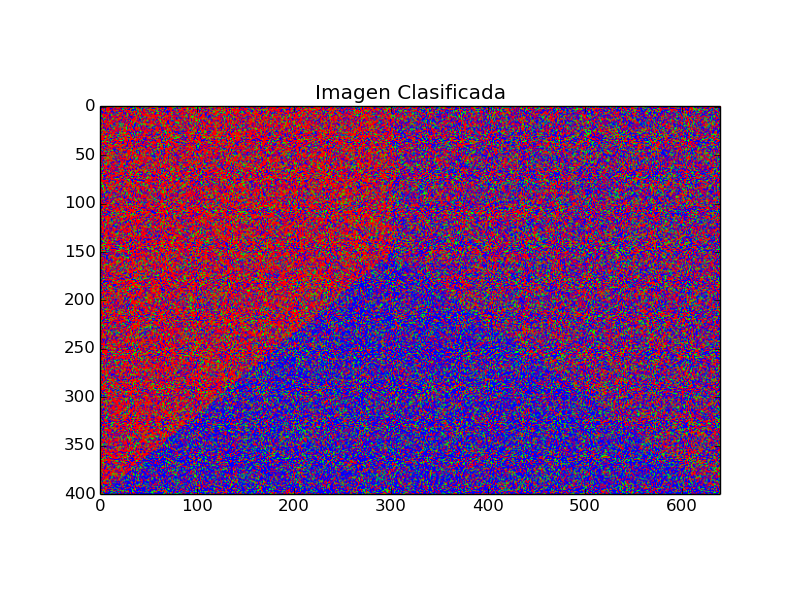
\includegraphics[width=0.45\textwidth]{img/ej2-caso1a-clfPhantom.png}
\caption{Caso 1. Ejemplo 1. A la izquierda los puntos sintéticos, con el color correspondiente al ground truth. A la derecha, la imagen clasificada.}
\label{ej2_caso1a}
\end{figure}

\begin{figure}[h!]
\centering
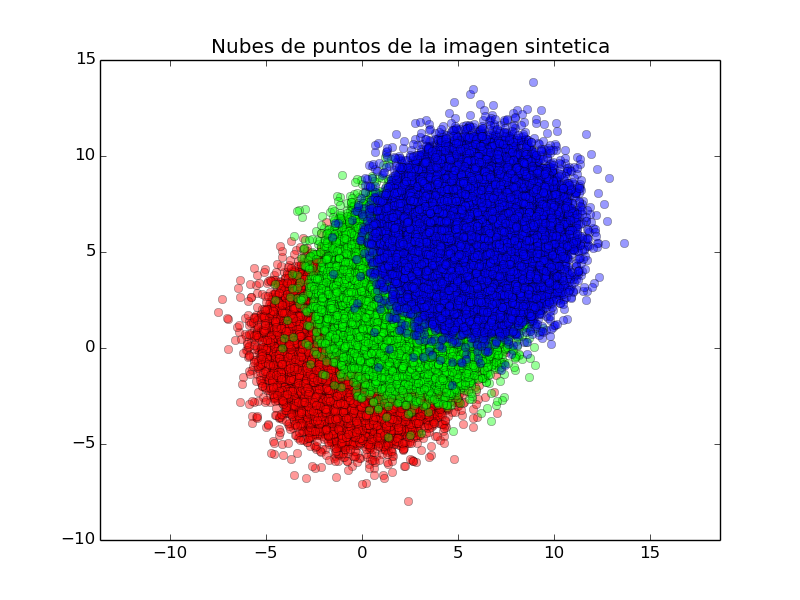
\includegraphics[width=0.45\textwidth]{img/ej2-caso1b-puntos.png}
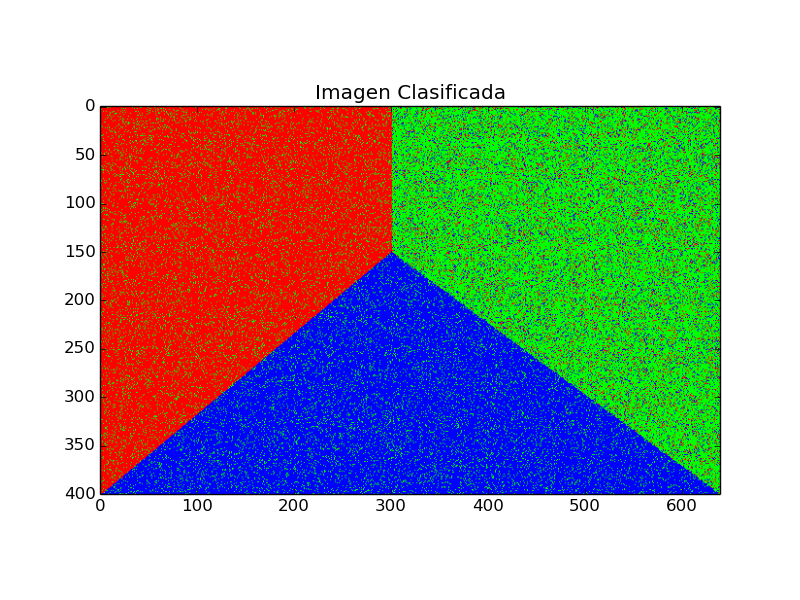
\includegraphics[width=0.45\textwidth]{img/ej2-caso1b-clfPhantom.png}
\caption{Caso 1. Ejemplo 2. A la izquierda los puntos sintéticos, con el color correspondiente al ground truth. A la derecha, la imagen clasificada.}
\label{ej2_caso1b}
\end{figure}

Comparando ambos ejemplos verificamos algo que era esperable: Cuanto más solapados estén los puntos (ejemplo 1), peor va a ser la clasificación, dado que es más difícil separarlos. En el ejemplo 1 los únicos colores que se distinguen son el azul y el rojo, ya que son las clases de las puntas (las más separadas, $C_1$ y $C_3$), mientras que la clase verde ($C_2$) quedó en el medio y muy pocos puntos fueron clasificados correctamente. Veamos las matrices de confusión:

\begin{tabular}{ r | c | c | c |}
    Ejemplo 1      &  {\color{red}$C_1$} & {\color{green}$C_2$} & {\color{blue}$C_3$} \\
  \hline
  Clasificado {\color{red}$C_1$}    &  48111         &     39298    & 21468 \\
  \hline
  Clasificado {\color{green}$C_2$}    &  12325          &     14921    & 11858\\
  \hline
  Clasificado {\color{blue}$C_3$}    &   22653            &     39351    & 46015\\
  \hline
  \% Acierto   & 57.90\% & 15.95\% & 58.00\% \\
  \hline
  \% Acierto Total & \multicolumn{3}{ c |}{42.60\%} \\
  \hline
\end{tabular}
\hspace{0.7cm}
\begin{tabular}{ r | c | c | c |}
    Ejemplo 2      &  {\color{red}$C_1$} & {\color{green}$C_2$} & {\color{blue}$C_3$} \\
  \hline
  Clasificado {\color{red}$C_1$}    &  73913         &     10232    & 12 \\
  \hline
  Clasificado {\color{green}$C_2$}    &  9170          &     72989    & 8816\\
  \hline
  Clasificado {\color{blue}$C_3$}    &   6            &     10349    & 70513\\
  \hline
  \% Acierto   & 88.96\% & 78.00\% & 88.87\% \\
  \hline
  \% Acierto Total & \multicolumn{3}{ c |}{84.93\%} \\
  \hline
\end{tabular}

Las matrices de confusión se condicen con lo que se observa en los gráficos. Además se ve claramente que en el ejemplo 2 los colores rojo y azul prácticamente no se mezclan (ambos se mezclan sólo con el verde, que es la clase que se solapa con ambos), mientras que la clase verde es la peor clasificada.


\subsection*{Caso 2: $\Sigma_i \neq \Sigma_j \ \forall i\neq j$, $\Sigma_k\propto I$}
Vamos a ver los mismos dos ejemplos, pero ahora las clases tendrán distintas matrices de covarianza. En ambos ejemplos vamos a tomar:
$$\Sigma_1 = \begin{pmatrix}10 & 0\\ 0 & 10\end{pmatrix}, \ \ \ \Sigma_2 = \begin{pmatrix}3 & 0\\ 0 & 3\end{pmatrix}, \ \ \ \Sigma_3 = \begin{pmatrix}1 & 0\\ 0 & 1\end{pmatrix}$$
Los valores de $\mu_k$ en ambos ejemplos se mantienen como en el {\bf Caso 1}. Los resultados se presentan en la Figuras \ref{ej2_caso2a} y \ref{ej2_caso2b}.

\begin{figure}[h!]
\centering
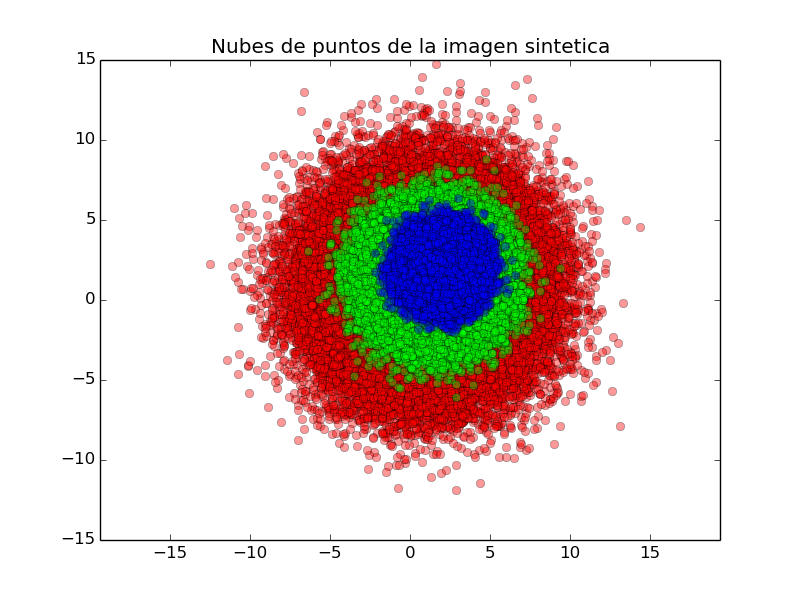
\includegraphics[width=0.45\textwidth]{img/ej2-caso2a-puntos.png}
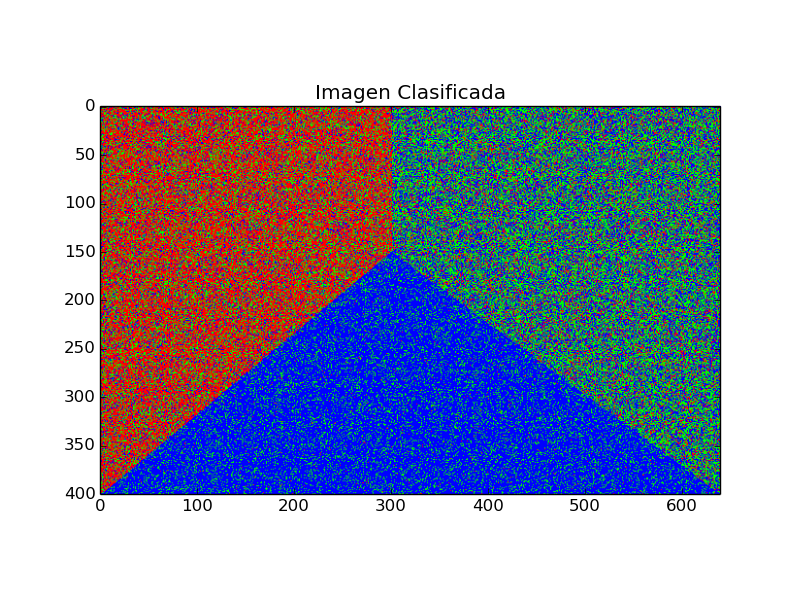
\includegraphics[width=0.45\textwidth]{img/ej2-caso2a-clfPhantom.png}
\caption{Caso 2. Ejemplo 1. A la izquierda los puntos sintéticos, con el color correspondiente al ground truth. A la derecha, la imagen clasificada.}
\label{ej2_caso2a}
\end{figure}

\begin{figure}[h!]
\centering
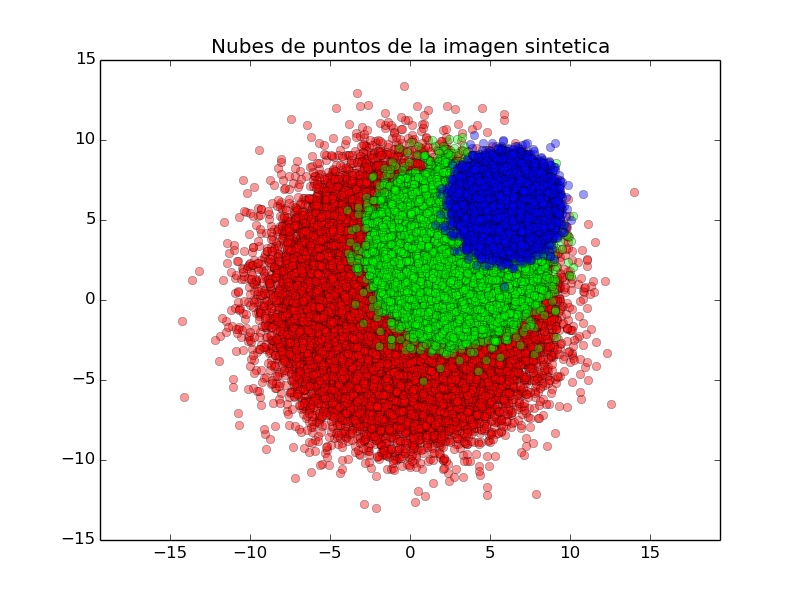
\includegraphics[width=0.45\textwidth]{img/ej2-caso2b-puntos.png}
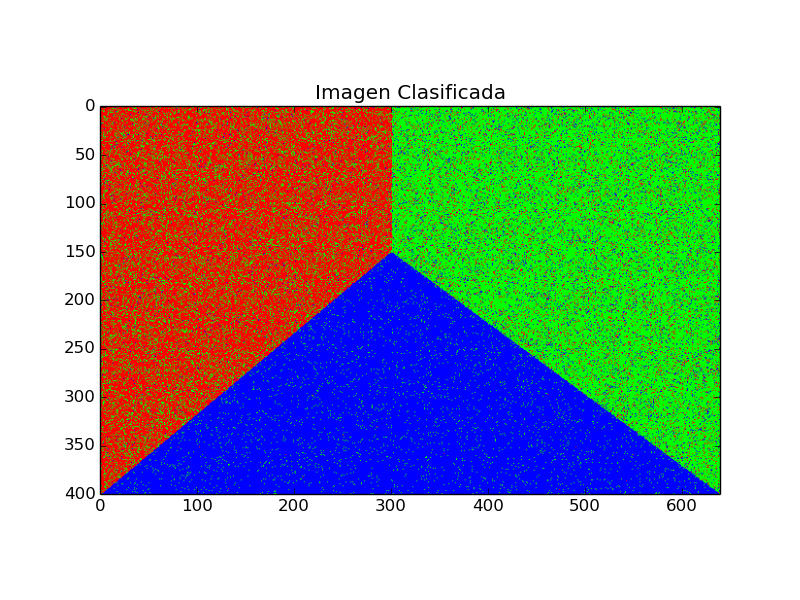
\includegraphics[width=0.45\textwidth]{img/ej2-caso2b-clfPhantom.png}
\caption{Caso 2. Ejemplo 2. A la izquierda los puntos sintéticos, con el color correspondiente al ground truth. A la derecha, la imagen clasificada.}
\label{ej2_caso2b}
\end{figure}

\begin{tabular}{ r | c | c | c |}
    Ejemplo 1      &  {\color{red}$C_1$} & {\color{green}$C_2$} & {\color{blue}$C_3$} \\
  \hline
  Clasificado {\color{red}$C_1$} & 50287 & 16366 & 547 \\
\hline
Clasificado {\color{green}$C_2$} & 20682 & 39585 & 13598 \\
\hline
Clasificado {\color{blue}$C_3$} & 12120 & 37619 & 65196 \\
\hline
\% Acierto & 60.52\% & 42.31\% & 82.17\% \\
\hline
\% Acierto Total & \multicolumn{3}{ c |}{60.57\%} \\
\hline
\end{tabular}
\hspace{0.7cm}
\begin{tabular}{ r | c | c | c |}
    Ejemplo 2      &  {\color{red}$C_1$} & {\color{green}$C_2$} & {\color{blue}$C_3$} \\
  \hline
  Clasificado {\color{red}$C_1$} & 64826 & 8884 & 14 \\
\hline
Clasificado {\color{green}$C_2$} & 17378 & 78240 & 2829 \\
\hline
Clasificado {\color{blue}$C_3$} & 885 & 6446 & 76498 \\
\hline
\% Acierto & 78.02\% & 83.62\% & 96.42\% \\
\hline
\% Acierto Total & \multicolumn{3}{ c |}{85.77\%} \\
\hline
\end{tabular}

Como puede observarse en los resultados, la clase $C_3$ (azul) fue la mejor clasificada en ambos casos, a pesar de estar superpuesta con las otras clases. Esto se debe a que tiene menor dispersión y la densidad de probabilidad se concentra alrededor de la media con valores muy altos, dando como resultado que las predicciones de puntos en la región de los puntos azules, sea siempre para la clase $C_3$. De hecho observar que en la fila de los puntos clasificados como $C_3$ hay muchos datos clasificados erróneamente, al punto que en el Ejemplo 1, hay casi tantos datos correctamente clasificados en $C_2$ como datos de $C_2$ que fueron clasificados como $C_3$.


\subsection{Caso 3: $\Sigma_k \ \cancel{\propto} I$}
En este caso consideraremos algunos ejemplos interesantes. En todos los ejemplos, definimos la matriz de covarianzas para la case $k$ como:
$$\Sigma_k=\begin{pmatrix}(\sigma_1^{(k)})^2 & \rho^k\sigma_1^{(k)}\sigma_2^{(k)} \\ \rho^{(k)}\sigma_1^{(k)}\sigma_2^{(k)} & (\sigma_2^{(k)})^2 \end{pmatrix}$$

\subsubsection{Ejemplo 1}
Tomamos $\mu_k = (0;0)^t$ y $\Sigma_k$ definida por
\begin{itemize}
  \item $\sigma_1^{(1)} = 50, \sigma_2^{(1)} = 50, \rho^{(1)}=0.4 $.
  \item $\sigma_1^{(2)} = 10, \sigma_2^{(2)} = 10, \rho^{(2)}=0.2 $.
  \item $\sigma_1^{(3)} = 2, \sigma_2^{(3)} = 2, \rho^{(3)}=-0.7 $.
\end{itemize}

Los resultados se presentan en la Figura \ref{ej1_caso3a} y la matriz de confusión quedó así:

\begin{tabular}{ r | c | c | c |}
    Ejemplo 2      &  {\color{red}$C_1$} & {\color{green}$C_2$} & {\color{blue}$C_3$} \\
  \hline
  Clasificado {\color{red}$C_1$} & 64826 & 8884 & 14 \\
\hline
Clasificado {\color{green}$C_2$} & 17378 & 78240 & 2829 \\
\hline
Clasificado {\color{blue}$C_3$} & 885 & 6446 & 76498 \\
\hline
\% Acierto & 78.02\% & 83.62\% & 96.42\% \\
\hline
\% Acierto Total & \multicolumn{3}{ c |}{85.77\%} \\
\hline
\end{tabular}

\begin{figure}[h!]
\centering
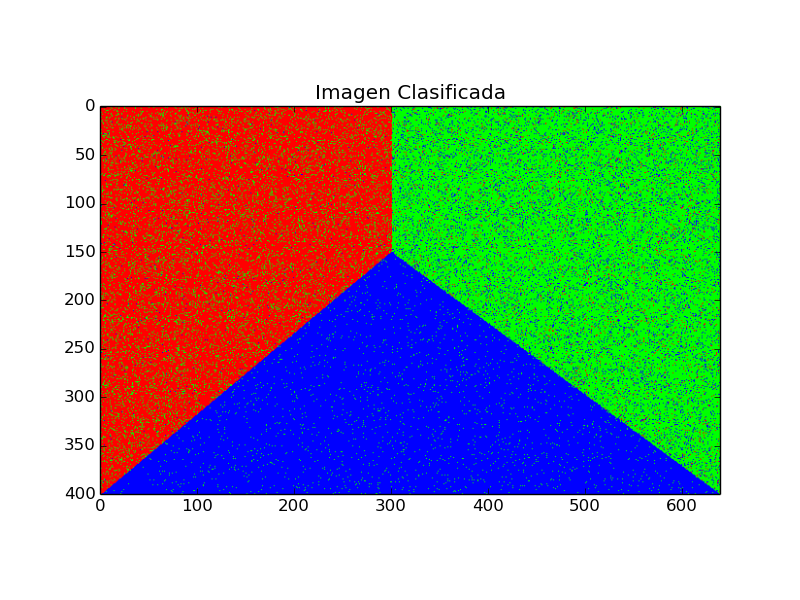
\includegraphics[width=0.45\textwidth]{img/ej2-caso3a-puntos.png}
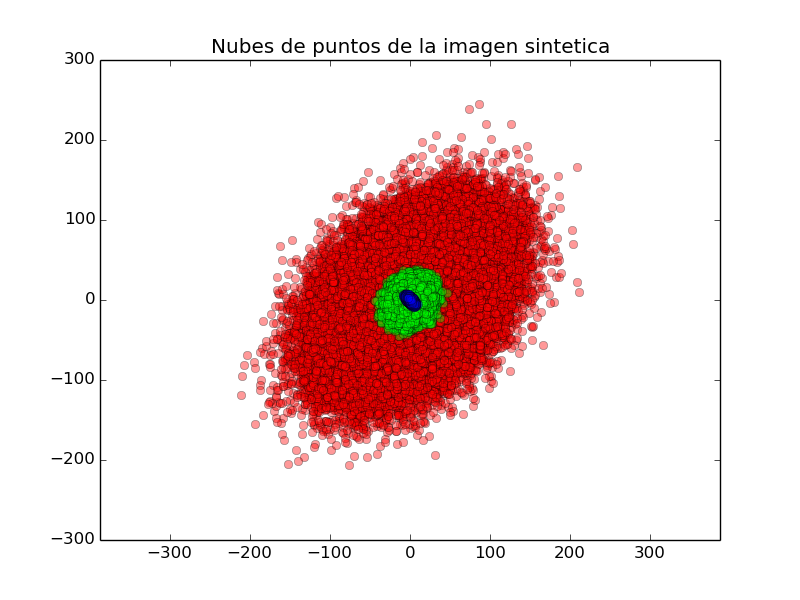
\includegraphics[width=0.45\textwidth]{img/ej2-caso3a-clfPhantom.png}
\caption{Caso 3. Ejemplo 1. A la izquierda los puntos sintéticos, con el color correspondiente al ground truth. A la derecha, la imagen clasificada.}
\label{ej2_caso3a}
\end{figure}

En este ejemplo se observa que si mantenemos la media de las distribuciones todas iguales pero las dispersiones son considerablemente distintas, se pueden obtener buenos resultados de clasificación. Esto demuestra que la calidad de la clasificación depende tanto de la media (como vimos en los ejemplos del {\bf Caso 1}) como de la matriz de covarianzas (a diferencia de los ejemplos observados en el {\bf Caso 2}).


\subsubsection{Ejemplo 2}
Mismas covarianzas que en el Ejemplo 1, pero ahora separamos los $\mu_k$:
\begin{itemize}
  \item $\mu_1 = (0;0)^t$.
  \item $\mu_2 = (-50;0)^t$.
  \item $\mu_3 = (40;40)^t$.
\end{itemize}

Los resultados se presentan en la Figura \ref{ej1_caso3b} y la matriz de confusión quedó así:

\begin{tabular}{ r | c | c | c |}
    Ejemplo 2      &  {\color{red}$C_1$} & {\color{green}$C_2$} & {\color{blue}$C_3$} \\
  \hline
  Clasificado {\color{red}$C_1$} & 75491 & 1975 & 63 \\
\hline
Clasificado {\color{green}$C_2$} & 7138 & 91595 & 0 \\
\hline
Clasificado {\color{blue}$C_3$} & 460 & 0 & 79278 \\
\hline
\% Acierto & 90.86\% & 97.89\% & 99.92\% \\
\hline
\% Acierto Total & \multicolumn{3}{ c |}{96.24\%} \\
\hline
\end{tabular}

\begin{figure}[h!]
\centering
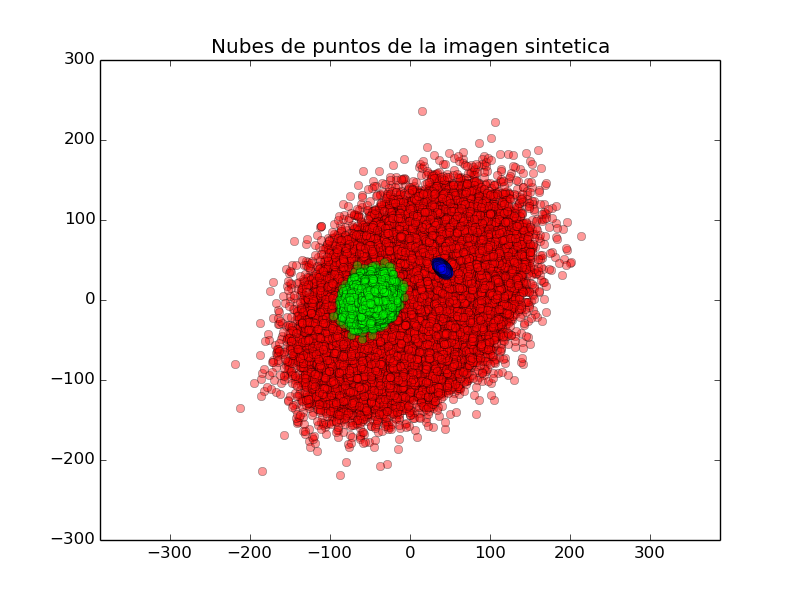
\includegraphics[width=0.45\textwidth]{img/ej2-caso3b-puntos.png}
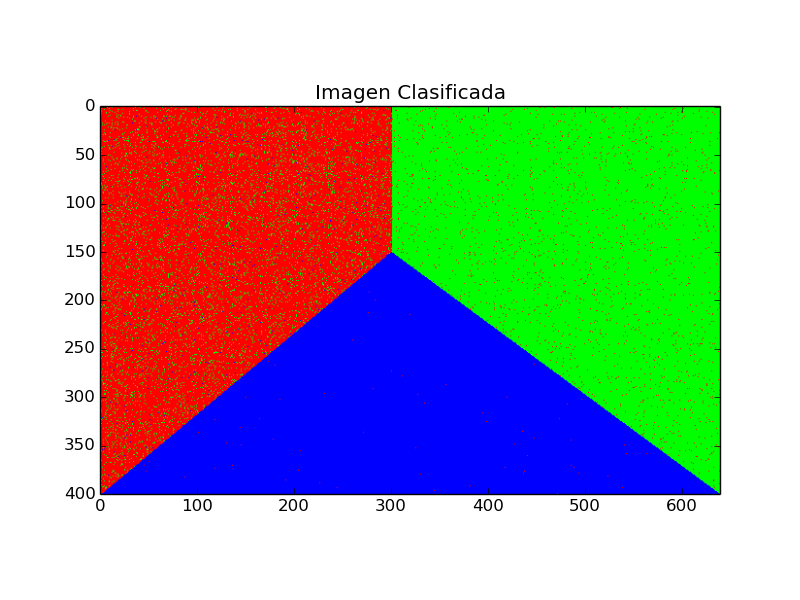
\includegraphics[width=0.45\textwidth]{img/ej2-caso3b-clfPhantom.png}
\caption{Caso 3. Ejemplo 2. A la izquierda los puntos sintéticos, con el color correspondiente al ground truth. A la derecha, la imagen clasificada.}
\label{ej2_caso3b}
\end{figure}

Observemos que al separar los valores medios aumentan más de un 10\% los aciertos totales, confirmando los razonamientos previos. En particular la clase azul ($C_3$) clasifica casi perfecta porque no se solapa con la densidad de la clase verde ($C_2$) y porque el solapamiento con la clase roja ($C_1$) se da en una región alejada de la media y con poca superficie (por la baja covarianza de $C_3$), entonces son pocos los puntos rojos que son clasificados como azules. En la imagen clasificada esto también se observa fácilmente ya que la región azul tiene muy poco ruido, mientras que las regiones verde y roja tienen muchos puntos intercambiados.

\subsection{Conclusiones}

En base a los casos analizados, comprobamos que el solapamiento de las nubes de puntos generan errores al clasificar. Además concluímos que aún en casos de solapamiento total se pueden obtener buenos clasificadores Bayesianos si
\begin{itemize}
  \item los valores medios están suficientemente separados y/o
  \item las dispersiones son considerablemente distintas.
\end{itemize}
Es decir que la diferencia en los parámetros de la distribución pesa más que el solapamiento a la hora de clasificar.


\section{Ejercicio 3: Clasificador Bayesiano en imagen real (con estimadores de m.v.)}

\begin{figure}[h!]
\centering
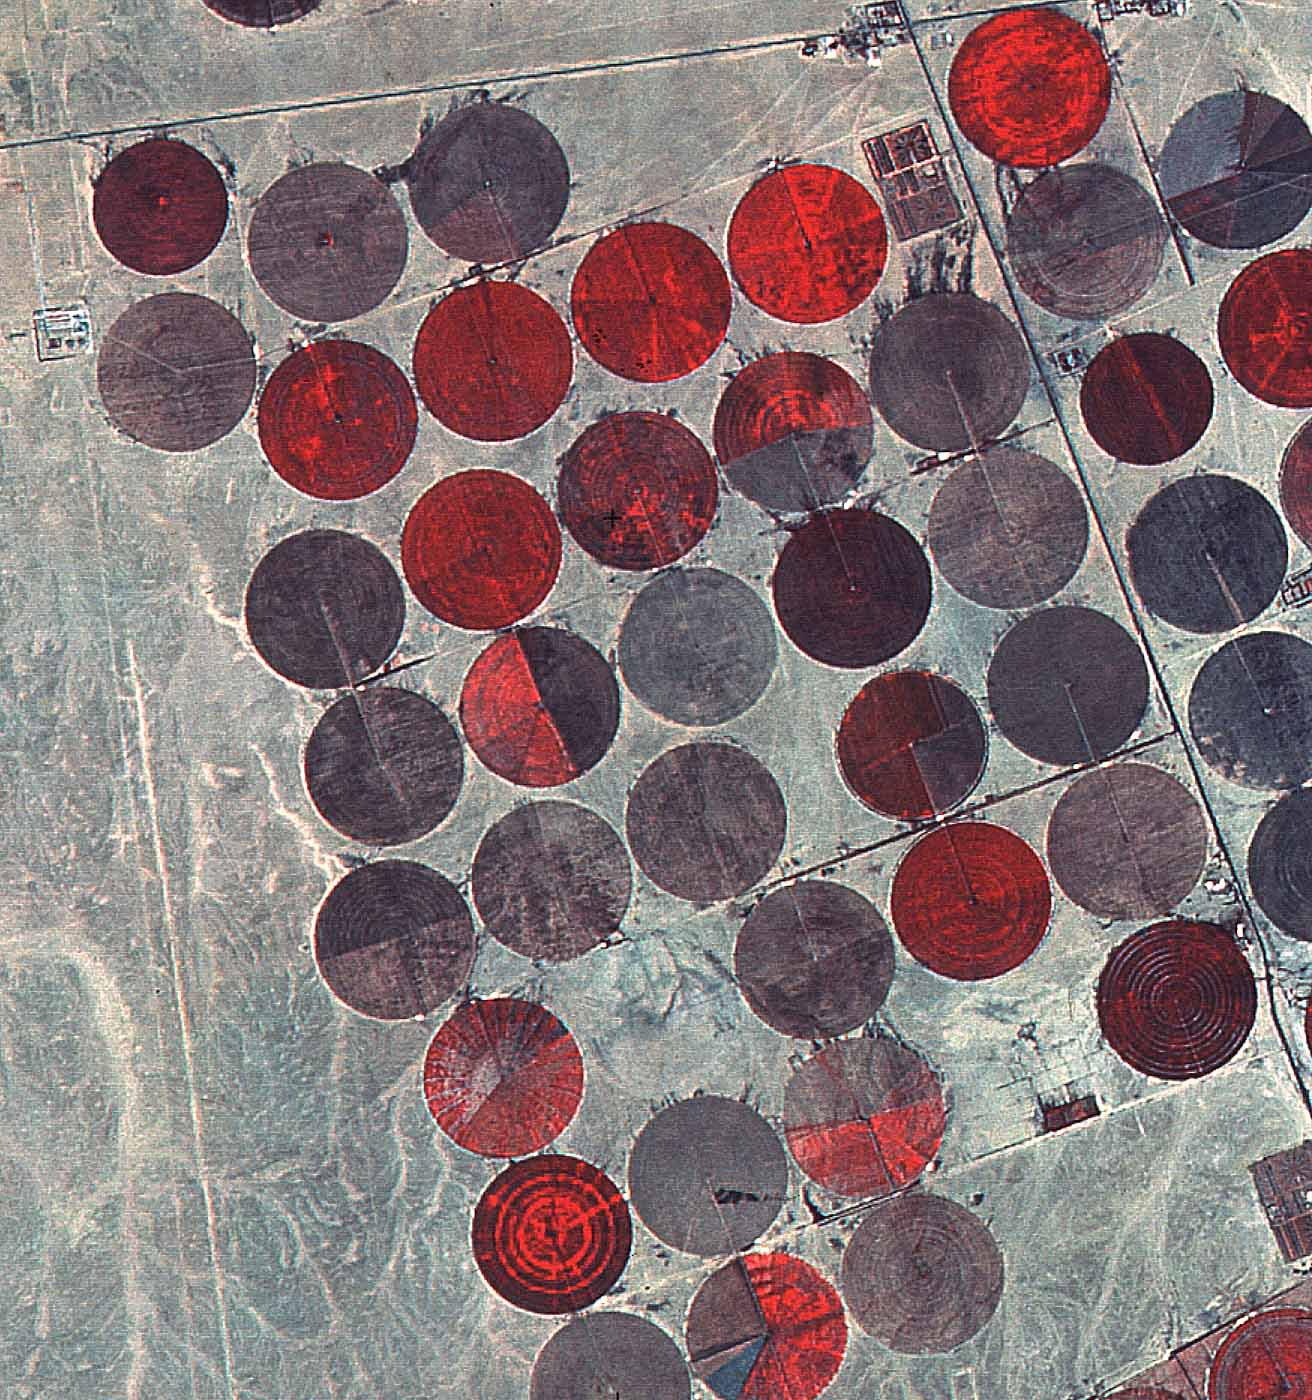
\includegraphics[width=0.4\textwidth]{img/circular.jpg}
\caption{Imagen {\tt circular.jpg}. $C_1$ desierto, $C_2$ cultivos grises, $C_3$ cultivos negros (o gris oscuro) y $C_4$ cultivos rojos.}
\label{circular}
\end{figure}


En este ejercicio vamos a tomar la imagen {\tt circular.jpg} (ver Figura \ref{circular}) e interpretar cada pixel $(i,j)$ RGB como un feature vector $x_{ij}\in\real^3$.
Vamos a crear un clasificador Bayesiano de pixels para las clases:
\begin{enumerate}
  \item[$C_1$:] Pixel correspondiente a desierto
  \item[$C_2$:] Pixel correspondiente a cultivo gris
  \item[$C_3$:] Pixel correspondiente a cultivo negro (o gris oscuro)
  \item[$C_4$:] Pixel correspondiente a cultivo rojo
\end{enumerate}
Para entrenar el clasificador utilizaremos distintas regiones de entrenamiento que vamos a extraer manualmente de la imagen. Asumiendo que las verosimilitudes $p(x|C_k)$ tienen distribución Normal $\mathcal{N}(\mu_k, \Sigma_k)$, vamos a realizar estimaciones de máxima verosimilitud para los parámetros $\mu_k \in\real^3$ y $\Sigma_k\in\real^{3\times 3}$. Luego usaremos estos valores en un clasificador Bayesiano,
suponiendo que las clases son equiprobables a priori ($P(C_i) = P(C_j) \ \forall i,j$). 
%para distintas probabilidades a priori.
Para analizar la calidad de la solución, calcularemos las matrices de confusión sobre regiones de entrenamiento y de prueba, y además generaremos una imagen clasificada, similar a la del ejercicio 2.

Para los experimentos, extrajimos 7 regiones de 50x50 pixels de cada clase $C_k$. Estas regiones las utilizaremos para entrenamiento y prueba.

\begin{figure}[h!]
\centering
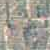
\includegraphics[width=0.13\textwidth]{img/regiones/C1_50x50_01.png}
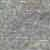
\includegraphics[width=0.13\textwidth]{img/regiones/C1_50x50_02.png}
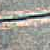
\includegraphics[width=0.13\textwidth]{img/regiones/C1_50x50_03.png}

\includegraphics[width=0.13\textwidth]{img/regiones/C1_50x50_04.png}
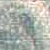
\includegraphics[width=0.13\textwidth]{img/regiones/C1_50x50_05.png}

\includegraphics[width=0.13\textwidth]{img/regiones/C1_50x50_06.png}

\includegraphics[width=0.13\textwidth]{img/regiones/C1_50x50_07.png}
\vspace{0.5cm}

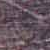
\includegraphics[width=0.13\textwidth]{img/regiones/C2_50x50_01.png}
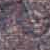
\includegraphics[width=0.13\textwidth]{img/regiones/C2_50x50_02.png}
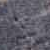
\includegraphics[width=0.13\textwidth]{img/regiones/C2_50x50_03.png}
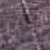
\includegraphics[width=0.13\textwidth]{img/regiones/C2_50x50_04.png}
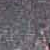
\includegraphics[width=0.13\textwidth]{img/regiones/C2_50x50_05.png}
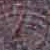
\includegraphics[width=0.13\textwidth]{img/regiones/C2_50x50_06.png}
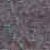
\includegraphics[width=0.13\textwidth]{img/regiones/C2_50x50_07.png}
\vspace{0.5cm}

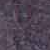
\includegraphics[width=0.13\textwidth]{img/regiones/C3_50x50_01.png}

\includegraphics[width=0.13\textwidth]{img/regiones/C3_50x50_02.png}
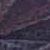
\includegraphics[width=0.13\textwidth]{img/regiones/C3_50x50_03.png}
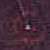
\includegraphics[width=0.13\textwidth]{img/regiones/C3_50x50_04.png}
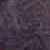
\includegraphics[width=0.13\textwidth]{img/regiones/C3_50x50_05.png}

\includegraphics[width=0.13\textwidth]{img/regiones/C3_50x50_06.png}
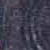
\includegraphics[width=0.13\textwidth]{img/regiones/C3_50x50_07.png}
\vspace{0.5cm}


\includegraphics[width=0.13\textwidth]{img/regiones/C4_50x50_01.png}

\includegraphics[width=0.13\textwidth]{img/regiones/C4_50x50_02.png}
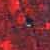
\includegraphics[width=0.13\textwidth]{img/regiones/C4_50x50_03.png}
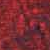
\includegraphics[width=0.13\textwidth]{img/regiones/C4_50x50_04.png}

\includegraphics[width=0.13\textwidth]{img/regiones/C4_50x50_05.png}
\includegraphics[width=0.13\textwidth]{img/regiones/C4_50x50_06.png}
\includegraphics[width=0.13\textwidth]{img/regiones/C4_50x50_07.png}
\caption{Regiones por cada clase. En la fila $k$ se encuentran las regiones para la clase $k$. Para cada clase enumeramos las regiones de 1 a 7, de izquierda a derecha}
\label{regiones}
\end{figure}

%Además en cada experimento vamos a considerar dos posibles probabilidades a priori:
%\begin{description}
%  \item[Equiprobables] $P(C_j) = P(C_i) \ \forall i,j$
%  \item[Proporcionales] Asignamos probabilidades proporcionales a la cantidad de píxels aproximado de cada clase.
%  \begin{itemize}
%    \item Dado que aproximadamente el 40\% de la imagen es desierto, tomamos $P(C_1) = 0.4$. Luego $P(cultivo) = 0.6$.
%    \item Para los cultivos contamos la cantidad de círculos completos (aproximadamente), y nos dió 41. Luego contamos cuántos eran de cada color y en función de esto determinamos las probabilidades a priori de las demás clases:
%     $$P(C_2) = \frac{12}{41}P(cultivo), \ \ \  P(C_3) = \frac{12}{41}P(cultivo), \ \ \  P(C_4) = \frac{17}{41}P(cultivo)$$
%  \end{itemize}

%\end{description}

\subsection{Experimento 1}
Tomamos la region 1 de cada clase como entrenamiento y las otras 6 regiones como prueba. Los resultados se presentan en la Figura \ref{ej3-caso1-equi}. %para el caso de probabilidades a priori equiprobables y en la Figura \ref{ej3-caso1-prop} para el caso de probabilidades a priori proporcionales.

Matrices de confusión para conjunto de entrenamiento (arriba) y prueba (abajo):

\begin{tabular}{ r | c | c | c | c |}
    Exp 1 (entrenamiento)     &  $C_1$ & $C_2$ & $C_3$ & $C_4$ \\
  \hline
Clasificado $C_1$ & 2483 & 16 & 0 & 0 \\
\hline
Clasificado $C_2$ & 17 & 2480 & 59 & 0 \\
\hline
Clasificado $C_3$ & 0 & 1 & 2441 & 0 \\
\hline
Clasificado $C_4$ & 0 & 3 & 0 & 2500 \\
\hline
\% Acierto & 99.32\% & 99.20\% & 97.64\% & 100.00\% \\
\hline
\% Acierto Total & \multicolumn{4}{ c |}{99.04\%} \\
\hline
\end{tabular}

\vspace{0.3cm}
\begin{tabular}{ r | c | c | c | c |}
    Exp 1 (prueba)     &  $C_1$ & $C_2$ & $C_3$ & $C_4$ \\
  \hline
Clasificado $C_1$ & 14891 & 1932 & 200 & 753 \\
\hline
Clasificado $C_2$ & 54 & 11445 & 4668 & 457 \\
\hline
Clasificado $C_3$ & 3 & 1577 & 8576 & 8 \\
\hline
Clasificado $C_4$ & 52 & 46 & 1556 & 13782 \\
\hline
\% Acierto & 99.27\% & 76.30\% & 57.17\% & 91.88\% \\
\hline
\% Acierto Total & \multicolumn{4}{ c |}{81.16\%} \\
\hline
\end{tabular}


\begin{figure}[h!]
\centering
\includegraphics[width=0.5\textwidth]{img/ej3-caso1-equi-puntos.png}

\includegraphics[width=0.3\textwidth]{img/ej3-caso1-equi-clasif.png}
\includegraphics[width=0.3\textwidth]{img/circular.jpg}
\caption{Experimento 1%(con $P(C_j)$ {\bf equiprobables})
. Arriba, 50 puntos de cada clase tomados aleatoriamente del conjunto de entrenamiento. Abajo la imagen {\tt circular.jpg} original comparada con la imagen clasificada.}
\label{ej3-caso1-equi}
\end{figure}

Por un lado, en el gráfico de puntos observamos que todos los puntos correspondientes a las clases $C_1$, $C_2$ y $C_3$ se encuentran en una especie de recta con dirección $(1,1,1)$ en $\real^3$. Esto tiene sentido dado que las tres clases corresponden a distintos niveles de grises y un gris en RGB se forma cuando $R=G=B$. Además vemos que los puntos de $C_1$ se encuentran más arriba dado que corresponden a un gris más claro (cercano al blanco, que en RGB es $(255,255,255)$) y los de $C_3$ se encuentran más abajo dado que corresponden a cultivos de color negro (negro en RGB es $(0,0,0)$). Los puntos de la clase $C_2$ están bastante mezclados con los de $C_3$ porque corresponden a un gris intermedio, tirando a oscuro. Los punto de $C_4$ corresponden a tonos de rojo, entonces se encuentran cerca del $(255,0,0)$ que corresponde al color rojo en RGB.

Por otro lado, observamos que usando una única imagen de entrenamiento por cada clase, obtuvimos un 80\% de aciertos y la imagen clasificada es muy similar a la imagen real. En la región de desierto hay error en la parte de las líneas negras (que fueron clasificadas como rojas). Además hay bastante confusión entre cultivos grises y negros, lo cual se observa gráficamente y numéricamente en los porcentajes de acierto de las clases $C_2$ y $C_3$ respectivamente; esto también se observa en la nube de puntos, que $C_2$ y $C_3$ están bastante mezclados.



\subsection{Experimento 2}
En este experimento vamos a agregar las siguientes regiones de entrenamiento:
\begin{itemize}
  \item Región 3 de $C_1$ ya que incluye una parte de línea negra que queremos clasificar como parte del desierto.
  \item Región 3 de $C_2$ ya que es un gris un poco más claro y permita evitar errores donde $C_2$ fue clasificada como desierto en el experimento 1.
  \item Región 2 de $C_3$ para ver si podemos separar mejor $C_2$ y $C_3$.
  \item Región 2 de $C_4$ para agregar la misma cantidad de puntos de todas las clase al conjunto de entrenamiento.
\end{itemize}
Las regiones de prueba son todas las que no son de entrenamiento. Los resultados se presentan en la Figura \ref{ej3-caso2-equi}. %para el caso de probabilidades a priori equiprobables y en la Figura \ref{ej3-caso1-prop} para el caso de probabilidades a priori proporcionales.

Matrices de confusión para conjunto de entrenamiento (arriba) y prueba (abajo):

\begin{tabular}{ r | c | c | c | c |}
    Exp 2 (entrenamiento)     &  $C_1$ & $C_2$ & $C_3$ & $C_4$ \\
  \hline
Clasificado $C_1$ & 4899 & 92 & 11 & 3 \\
\hline
Clasificado $C_2$ & 73 & 4228 & 521 & 5 \\
\hline
Clasificado $C_3$ & 4 & 680 & 4468 & 3 \\
\hline
Clasificado $C_4$ & 24 & 0 & 0 & 4989 \\
\hline
\% Acierto & 97.98\% & 84.56\% & 89.36\% & 99.78\% \\
\hline
\% Acierto Total & \multicolumn{4}{ c |}{92.92\%} \\
\hline
\end{tabular}

\vspace{0.3cm}
\begin{tabular}{ r | c | c | c | c |}
    Exp 2 (prueba)     &  $C_1$ & $C_2$ & $C_3$ & $C_4$ \\
  \hline
Clasificado $C_1$ & 12391 & 520 & 7 & 809 \\
\hline
Clasificado $C_2$ & 109 & 10868 & 4948 & 630 \\
\hline
Clasificado $C_3$ & 0 & 1095 & 7003 & 23 \\
\hline
Clasificado $C_4$ & 0 & 17 & 542 & 11038 \\
\hline
\% Acierto & 99.13\% & 86.94\% & 56.02\% & 88.30\% \\
\hline
\% Acierto Total & \multicolumn{4}{ c |}{82.60\%} \\
\hline
\end{tabular}


\begin{figure}[h!]
\centering
\includegraphics[width=0.5\textwidth]{img/ej3-caso2-equi-puntos.png}

\includegraphics[width=0.3\textwidth]{img/ej3-caso2-equi-clasif.png}
\includegraphics[width=0.3\textwidth]{img/circular.jpg}
\caption{Experimento 2%(con $P(C_j)$ {\bf equiprobables})
. Arriba, 50 puntos de cada clase tomados aleatoriamente del conjunto de entrenamiento. Abajo la imagen {\tt circular.jpg} original comparada con la imagen clasificada.}
\label{ej3-caso2-equi}
\end{figure}

En este caso empeoraron los aciertos en el conjunto de entrenamiento, aunque esto podría ser algo bueno si en el experimento 1 teníamos \emph{overfitting}. El porcentaje de aciertos total para el conjunto de pruebas subió muy poco. En la imagen clasificada vemos que algunas líneas del desierto están menos rojas pero sigue habiendo líneas rojas en el desierto.


\newpage
\subsection{Experimento 3}
En este experimento agregamos las regiones 2, 5, 4 y 5 para las clases $C_1$, $C_2$, $C_3$ y $C_4$ respectivamente.
Las regiones de prueba son todas las que no son de entrenamiento. Los resultados se presentan en la Figura \ref{ej3-caso3-equi}. %para el caso de probabilidades a priori equiprobables y en la Figura \ref{ej3-caso1-prop} para el caso de probabilidades a priori proporcionales.

Matrices de confusión para conjunto de entrenamiento (arriba) y prueba (abajo):

\begin{tabular}{ r | c | c | c | c |}
    Exp 3 (entrenamiento)     &  $C_1$ & $C_2$ & $C_3$ & $C_4$ \\
  \hline
Clasificado $C_1$ & 7348 & 152 & 12 & 0 \\
\hline
Clasificado $C_2$ & 104 & 6381 & 587 & 4 \\
\hline
Clasificado $C_3$ & 4 & 963 & 6820 & 64 \\
\hline
Clasificado $C_4$ & 44 & 4 & 81 & 7432 \\
\hline
\% Acierto & 97.97\% & 85.08\% & 90.93\% & 99.09\% \\
\hline
\% Acierto Total & \multicolumn{4}{ c |}{93.27\%} \\
\hline
\end{tabular}

\vspace{0.3cm}
\begin{tabular}{ r | c | c | c | c |}
    Exp 3 (prueba)     &  $C_1$ & $C_2$ & $C_3$ & $C_4$ \\
  \hline
Clasificado $C_1$ & 9893 & 236 & 4 & 690 \\
\hline
Clasificado $C_2$ & 103 & 8143 & 398 & 412 \\
\hline
Clasificado $C_3$ & 4 & 1584 & 9461 & 167 \\
\hline
Clasificado $C_4$ & 0 & 37 & 137 & 8731 \\
\hline
\% Acierto & 98.93\% & 81.43\% & 94.61\% & 87.31\% \\
\hline
\% Acierto Total & \multicolumn{4}{ c |}{90.57\%} \\
\hline
\end{tabular}


\begin{figure}[h!]
\centering
\includegraphics[width=0.5\textwidth]{img/ej3-caso3-equi-puntos.png}

\includegraphics[width=0.3\textwidth]{img/ej3-caso3-equi-clasif.png}
\includegraphics[width=0.3\textwidth]{img/circular.jpg}
\caption{Experimento 3%(con $P(C_j)$ {\bf equiprobables})
. Arriba, 50 puntos de cada clase tomados aleatoriamente del conjunto de entrenamiento. Abajo la imagen {\tt circular.jpg} original comparada con la imagen clasificada.}
\label{ej3-caso3-equi}
\end{figure}

En este caso obtuvimos una mejora considerable en el porcentaje de aciertos en los casos de prueba. Esto posiblemente se deba a que tenemos mayor dispersión en los datos de entrenamiento (comparar los puntos de la Figura \ref{ej3-caso3-equi} con la \ref{ej3-caso2-equi}) por haber usado más variedad de regiones de cada clase. También mejoró bastante la imagen clasificada, habiedo círculos que ahora fueron clasificados como negros o grises y antes eran clasificados erróneamente como grises o desierto, respectivamente.

A continuación presentamos una figura comparativa entre las imágenes clasificadas de cada experimento, para notar la evolución en las predicciones:

\begin{figure}[h!]
\centering
\includegraphics[width=0.3\textwidth]{img/circular.jpg}

\includegraphics[width=0.3\textwidth]{img/ej3-caso1-equi-clasif.png}
\includegraphics[width=0.3\textwidth]{img/ej3-caso2-equi-clasif.png}
\includegraphics[width=0.3\textwidth]{img/ej3-caso3-equi-clasif.png}

\caption{Arriba la imagen {\tt circular.jpg} original. Abajo los tres experimentos en orden de izquierda a derecha.}
\label{ej3-integrado}
\end{figure}

\newpage
\subsection{Experimento 4}
En este último experimento usamos todas las regiones como entrenamiento únicamente para observar si conseguíamos una mejora con respecto al experimento 3, pero como se observa en la Figura \ref{ej3-caso4}, prácticamente no hay diferencias.

\begin{figure}[h!]
\centering
\includegraphics[width=0.3\textwidth]{img/circular.jpg}

\includegraphics[width=0.3\textwidth]{img/ej3-caso3-equi-clasif.png}
\includegraphics[width=0.3\textwidth]{img/ej3-caso4-equi-clasif.png} 

\caption{Arriba la imagen {\tt circular.jpg} original. Abajo el experimento 3 a la izquierda y el experimento 4 a la derecha.}
\label{ej3-caso4}
\end{figure}


\section{Conclusiones}
Estudiamos en detalle el clasificador Bayesiano, llegando a las siguientes conclusiones:
\begin{itemize}
\item Las diferencias en media y dispersión de cada clase influye directamente en la calidad de las predicciones. Clases con distribuciones muy diferentes son más fáciles de separar y por lo tanto la clasificación de nuevos puntos es más precisa.
\item A pesar de ser el método más intuitivo y sencillo, a pesar de que haya clasificadores mucho más poderosos y robustos, el clasificador Bayesiano arrojó muy buenos resultados en la clasificación del Ejemplo 3. Siendo un método sencillo de implementar y eficiente al clasificar, es importante saber que en ciertos casos es un buen clasificador.
\end{itemzie}

\end{document}
